
%(BEGIN_QUESTION)
% Copyright 2014, Tony R. Kuphaldt, released under the Creative Commons Attribution License (v 1.0)
% This means you may do almost anything with this work of mine, so long as you give me proper credit

Calculate the amount of voltage between test points TP1 and TP3, and also the amount of voltage between test points TP2 and TP4:

$$\includegraphics[width=15.5cm]{i01157x01.eps}$$

$V_{TP1-TP3}$ = \hskip 40pt $V_{TP2-TP4}$ = 

\vskip 10pt

\underbar{file i01157}
%(END_QUESTION)





%(BEGIN_ANSWER)

$V_{TP1-TP3}$ = 15.83 volts \hskip 20pt $V_{TP2-TP4}$ = 22.22 volts

%(END_ANSWER)





%(BEGIN_NOTES)

Ask your students to explain how they obtained their answers.  There is more than one correct way to answer this question!

%INDEX% Electronics review: series and parallel circuits

%(END_NOTES)


